\documentclass[twoside,10pt]{article}
\usepackage{shlists}
\usepackage[spanish]{babel}
\usepackage[applemac]{inputenc}
\usepackage[T1]{fontenc}

\usepackage{multicol}
\usepackage{picinpar}

\usepackage{url}
\newcounter{vol}
\newcounter{num}
\newcounter{anyo}
\setcounter{vol}{8}
\setcounter{num}{1}
\setcounter{anyo}{2015}
\newcommand{\mes}{Enero}
\usepackage{revisionNLcol}


\title{Docencia 2.0\\ \large Juan Juli\'an Merelo, Fernando 
Tricas}
\author{\LARGE Paseando por las nubes}


\date{}

\AutTit{Docencia 2.0}

\begin{document}
\addtocounter{page}{2}

\maketitle
\vspace*{-8ex}

\begin{multicols}{2}


\vspace{1ex} {\small{\begin{window}[0,r,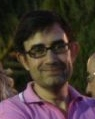
\includegraphics[width = 27
mm]{JJM.jpg},] \noindent\emph{JJ Merelo} es catedr\'{a}tico de Universidad
en el \'area de Arquitectura y Tecnolog\'{\i}a de Computadores. Usa,
desarrolla y promueve el software libre y todo tipo de conocimiento
abierto. 
\end{window}}}

\medskip

{\small{\begin{window}[0,r,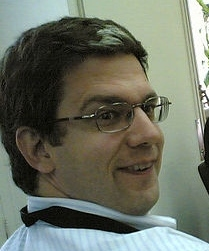
\includegraphics[width = 27 mm]{FTricas1.jpg},]
		\noindent \emph{Fernando Tricas Garc\'{\i}a} es profesor
		titular de Lenguajes y Sistemas Inform\'{a}ticos del Departamento
		de Inform\'{a}tica e Ingenier\'{\i}a de Sistemas de la Universidad de
		Zaragoza.  Empez\'{o} a estudiar la blogosfera casi cuando a\'{u}n no
		exist\'{\i}a (all\'{a} por el a\~{n}o 2002) y a tratar de integrarla en los
		cursos y tareas docentes un poco despu\'{e}s.  Ha impartido
		numerosas charlas relacionadas con el tema de la Web 2.0, 
		internet y universidad,\ldots\ 
		Es actualmente Vicerrector de Tecnolog\'{\i}as de la Informaci\'{o}n y
de la Comunicaci\'{o}n.   
		\end{window}}}



\bigskip

\noindent\emph{Todas las columnas de la serie Docencia 2.0
pueden descargarse en formato LaTeX desde
{\small\url{https://github.com/ReVision-Docencia-20/Columnas}}}

\noindent\rule{90mm}{1pt}

{\small \noindent
\includegraphics[height = 4ex]{CC.jpg} 2015 JJ. Merelo, F. Tricas. Este art\'{\i}culo es de acceso libre distribuido bajo los t\'erminos
de la Licencia Creative Commons de Atribuci\'on, que permite copiar,
distribuir y comunicar p\'ublicamente la obra en cualquier medio, s\'olido
o electr\'onico, siempre que se acrediten a los autores y fuentes
originales}


% \begin{thebibliography}{9}
% 	\bibitem{WA} John Paczkowski: \emph{WhatsApp: Bigger Than Twitter}.
% {\small\url{http://allthingsd.com/20130416/whatsapp-bigger-than-twitter/}},
% consultado en abril de 2013.}
% 
% \bibitem{Micr} Europa Press: Microsoft confirma la
% desaparici�n de Messenger y su integraci�n en Skype.
% {\small\texttt{http://www.europapress.es/portaltic/social 
% media/noticia-microsoft-confirma-desapari
% cion-messenger-integracion-skype-20121106
% 194539.html}},
% consultado en abril de 2013.
% 
% \bibitem{MT} Juan J. Merelo, F. Tricas:  \emph{Los medios y los memes.} En La
% Comunicaci�n Digital, editado por Germ�n Llorca Abad, Mar Iglesias
% Garc�a, �lvar Peris Blanes.  Tirant lo Blanc.  Valencia, Espa�a.
% pp.~219 -- 226.  2012.
% 
% \end{thebibliography}
\end{multicols}
\end{document}
	








\end{multicols}
\end{document}
�
